\section{Target Estimation} \label{sec:target_estimation}
Using the information gathered from the different models described in the sections before, the target estimation is determined. This target estimate is then used to go towards then influences the Filter/Gain block. Two different models are discussed and implemented. The first model that will be discussed is the Power Spectral Subtraction.

\subsection{Power Spectral Subtraction}
By transforming Eq. \ref{eq:psds1} into Eq. \ref{eq:psds2} and doing some manipulations Eq. \ref{eq:psds3} can be determined. This signal however has no phase associated with it. As the phase has not been changed, the original phase can be multiplied with it to end up with Eq. \ref{eq:psds4}.
\begin{align}
  P_{SS,k}(l) &= P_{YY,k}(l) - P_{NN,k}(l)
  \label{eq:psds1} \\
  \widehat{\abs{S_{k}(l)}}^{2} &= \abs{Y_{k}(l)}^{2}-\abs{N_{k}(l)}^{2}
  \label{eq:psds2} \\
  \widehat{\abs{S_{k}(l)}} &=
  \left(\max{\left\{1-\frac{E\left[\abs{N_{k}(l)}^{2}\right]}{\abs{y_{k}(l)}^{2}},\epsilon\right\}}\right)^{\frac{1}{2}}\abs{y_{k}(l)}
  \label{eq:psds3} \\
  S_{k}(l) &= \widehat{\abs{S_{k}(l)}} \cdot e^{j\measuredangle y_{k}(l)}
  \label{eq:psds4}
\end{align}

The results with Power Spectral Subtraction implemented can be seen in Fig. \ref{fig:PSS}. Spikes can be seen in the error plot when high the speech signal has high signal power.

\begin{figure}[h]
	\centering
	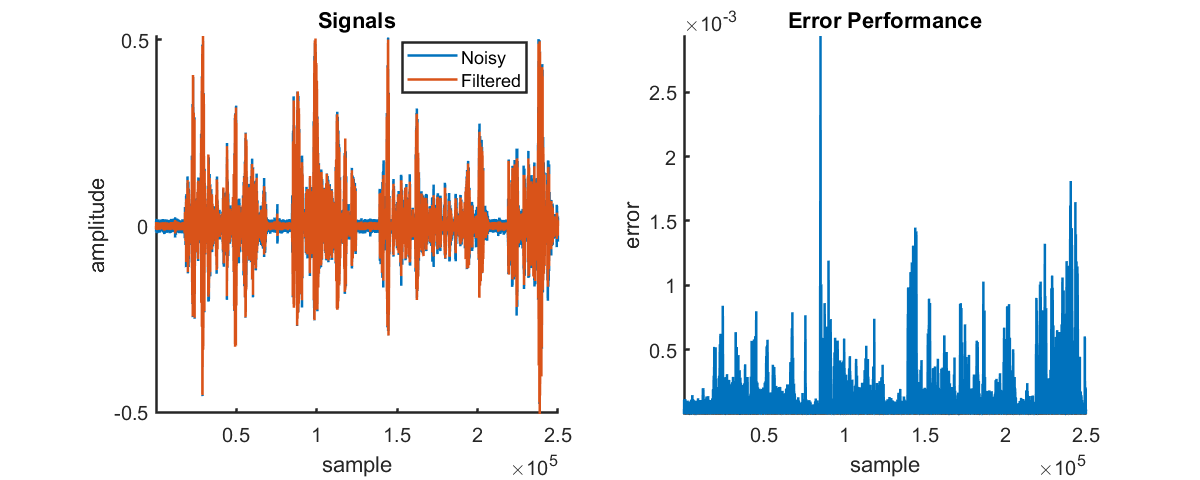
\includegraphics[width=\textwidth]{images/spectral_substraction.png}
	\caption{Results when performing Power Spectral Subtraction using Minimum Statistics Method and $\text{SNR}_{\text{dd}}$.}
	\label{fig:PSS}
\end{figure}
\clearpage

\subsection{Wiener filter}
The second implemented method is the Wiener filter. The Wiener filter uses the Signal-to-Noise Ratio to determine a gain, Eq. \ref{eq:wiener2} and Eq. \ref{eq:wiener3}, with which the noise speech signal is multiplied as can be seen Eq. \ref{eq:wiener1}.
\begin{align}
  \hat{S_{k}} &= H_{k} \cdot Y_{k}
  \label{eq:wiener1} \\
  H_{k} &= \frac{P_{SY,k}}{P_{PYY,k}}
  \label{eq:wiener2} \\
  &= \frac{SNR_{k}}{SNR_{k}+1}
  \label{eq:wiener3}
\end{align}

The results for the implementation of the Wiener Filter can be found in Fig. \ref{fig:Wiener}. The Wiener filter greatly reduces the noise in the parts where no speech is present. However, when speech is present the error seen is much bigger (10 times) than for the Power Spectral Subtraction. Which degrades the Speech Signal.
\begin{figure}[h]
	\centering
	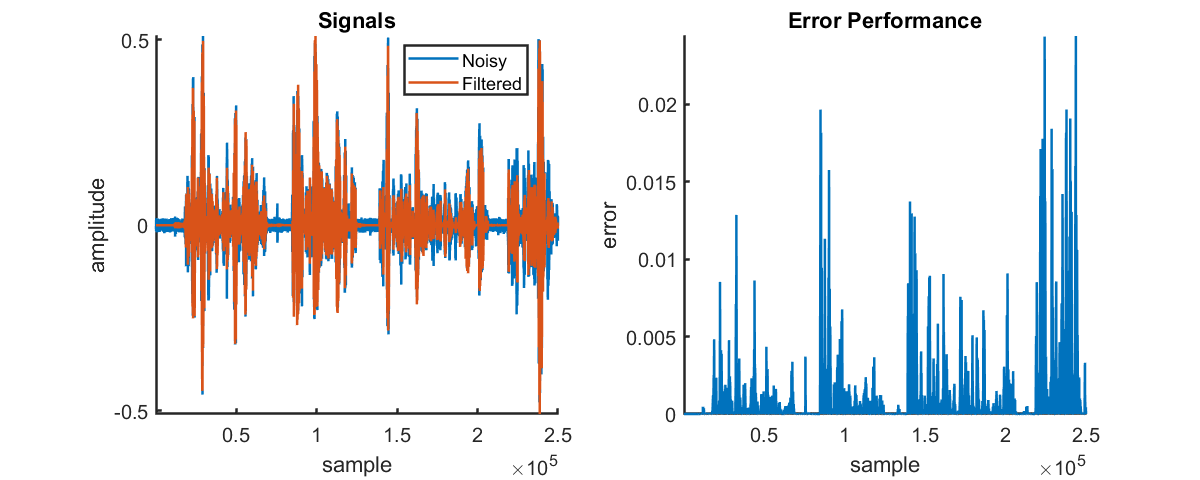
\includegraphics[width=\textwidth]{images/wiener.png}
	\caption{Results when using the Wiener Filter with Minimum Statistics Method and $\text{SNR}_{\text{dd}}$.}
	\label{fig:Wiener}
\end{figure}

